% !TEX encoding = UTF-8 Unicode
% !TEX spellcheck = es_ES

% Plantilla para el Trabajo de Fin de Grado/Máster de la Escuela Técnica 
% Superior de Ingenieros Navales de la Universidad Politécnica de Madrid.
% Esta plantilla está basada en la propuesta por el centro 
% en su página web en formato Microsoft Word.
% 
% Los planes para los que es aplicable son:
% - GRADO EN ARQUITECTURA NAVAL (GAN - XXX)
% - GRADO EN INGENIERÍA MARÍTIMA (GIM - XXX)
% - MÁSTER EN INGENIERÍA NAVAL Y OCEÁNICA (MINO - XXX)
% 
% ricardo.lopezg@alumnos.upm.es
% noviembre 2018
%
% PARA SIMPLIFICAR, EL PREÁMBULO ES UN DOCUMENTO SEPARADO
\documentclass[11pt,a4paper,twoside,openright]{report} 
%
%
%
% MÁRGENES
\usepackage[top=3.0cm, bottom=2.5cm, right=1.75cm,left=3.0cm,asymmetric]{geometry}
%
%
%
% PAQUETEs DE FUENTES Y ESTILOS
\usepackage{helvet}
\usepackage[utf8]{inputenc}
\usepackage[spanish,es-nodecimaldot]{babel}
\renewcommand{\familydefault}{\sfdefault}
\usepackage{courier}
\frenchspacing 
\setlength{\parindent}{0pt}
\setlength{\parskip}{6pt}
%
\usepackage[compact]{titlesec}
\titlespacing{\section}{0pt}{2ex}{1ex}
\titlespacing{\subsection}{0pt}{1ex}{0ex}
\titlespacing{\subsubsection}{0pt}{0.5ex}{0ex}
\usepackage{appendix}
%
%
%
% ENCABEZADO Y PIE DE PÁGINA
\usepackage{fancyhdr}
	\pagestyle{fancy}
\headheight=1.0cm
\renewcommand{\headrulewidth}{0pt}
\renewcommand{\chaptermark}[1]{\markboth{#1}{}}
\rhead{ \begin{picture}(0,0) \put(-30,-15){\includegraphics[width=2.2cm]{photos/etsin.png}} \end{picture}}
\lhead{\begin{picture}(0,0) \put(-60,-1){\includegraphics[width=3.5cm]{photos/poli.png}} \end{picture}}
\chead{hola}
\fancyfoot[C]{\thepage}
\fancypagestyle{plain}{}
\fancyhf{} 
\fancyhead[C]{\vfill \MakeUppercase \leftmark}
\rhead{ \begin{picture}(0,0) 		  \put(-30,-15){\includegraphics[width=2.2cm]{images/template/etsin.png}} \end{picture}}
\lhead{\begin{picture}(0,0) \put(-60,-1){\includegraphics[width=3.5cm]{images/template/poli.png}} \end{picture}}
\fancyfoot[C]{\thepage} 
%
%
%
% PAQUETES DE IMÁGENES
\usepackage{graphicx} % Para poner gráficos
\usepackage{xcolor}
\usepackage{lipsum}
\usepackage{epstopdf}
\usepackage{epsfig}
\usepackage{epsf}
\usepackage{float}
\usepackage{wrapfig}
\usepackage{lscape}
\usepackage{rotating}
%
%
%
% ENLACES DENTRO DEL DOCUMENTO
\usepackage{booktabs}
\usepackage{xcolor}	
\usepackage{subfigure}
\usepackage{mdframed}
\usepackage{hyperref}
\hypersetup{
	colorlinks   = true,
	linkcolor 	 = blue,
	urlcolor     = blue,
	citecolor    = blue
}
%
%
%
% MISCELÁNEO
\newcommand{\HRule}{\rule{\linewidth}{0.5mm}}
\usepackage{pdfpages}
\usepackage[usenames,dvipsnames]{pstricks}
\usepackage{cite} 
%
%
%
% EXPRESIONES MATEMÁTICAS
\usepackage{amsmath,amssymb,amsfonts,latexsym,cancel} 
\usepackage[math]{blindtext}
%
%
%
% PAQUETES PARA RENOMBRAR A CASTELLANO LOS ELEMENTOS (NO TODOS SON SIEMPRE NECESARIOS)
\renewcommand{\appendixname}{Anexo}
\renewcommand{\spanishtablename}{Tabla}
\renewcommand{\spanishlistfigurename}{Lista de figuras}
\renewcommand{\spanishlisttablename}{Lísta de tablas}
%\renewcommand{\contentsname}{Contenido}
%\renewcommand{\partname}{Parte}
%\renewcommand{\abstractname}{Resumen}
%\renewcommand{\refname}{Bibliografía}
%\renewcommand{\figurename}{Figura}
%
%
%
% INTRODUCIR CÓDIGOS 
\usepackage{listings}
\usepackage{showexpl}[rframe=none]
\definecolor{dkgreen}{rgb}{0,0.6,0}
\definecolor{gray}{rgb}{0.5,0.5,0.5}
\definecolor{mauve}{rgb}{0.58,0,0.82}
\lstset{ %
  language=[LaTeX]TeX,                 
  basicstyle=\small \ttfamily,
  numbers=left,                   
  numberstyle=\tiny\color{gray},   
  stepnumber=1,                    
  numbersep=5pt,                   
  backgroundcolor=\color{white}, 
  showspaces=false,                
  showstringspaces=false,        
  showtabs=false,                  
  frame=single,                   
  rulecolor=\color{black},        
  tabsize=4,                     
  captionpos=b,                 
  breaklines=true,               
  breakatwhitespace=false,       
  keywordstyle=\bfseries \color{blue},         
  commentstyle=\color{dkgreen},      
  stringstyle=\color{mauve},        
  escapeinside={\%*}{*)},          
  morekeywords={*,...}                
}


% INFORMACIÓN DEL DOCUMENTO (ACTUALIZA PORTADA)
\def\myauthor{(NOMBRE DEL AUTOR)}
\def\mytutor{(NOMBRE DEL TUTOR)}
\def\mycotutor{(NOMBRE DEL CO-TUTOR)}
\def\mydegree{GRADO EN \\ ARQUITECTURA NAVAL}
\def\mycode{GAN - XXX}
\def\mytitle{(TÍTULO DEL TRABAJO)}
\def\mydate{(MES Y AÑO DE LA PRESENTACIÓN)}
	
\begin{document}
	% PORTADA
	% !TEX encoding = UTF-8 Unicode
% !TEX root = GANXXX.tex
% !TEX spellcheck = es_ES
%%=========================================
\newgeometry{top=1cm, bottom=1.5cm, right=1.25cm,left=1.25cm}

\begin{titlepage}
	\begin{center}
		% Upper part of the page
		\includegraphics[width=0.4\textwidth]{images/template/upm.png}
		
		
		\vspace{1pc}
		\Large{UNIVERSIDAD POLITÉCNICA DE MADRID}
		
		
		\vspace{1pc}
		\Large{ \bfseries{ Escuela Técnica Superior \\ de Ingenieros Navales}}
		
		
		\vspace{1pc}
		\large{MADRID}
		
		
		\vspace{1pc}
		\textsc{\large TRABAJO DE FIN DE \mydegree}
		
		
		\vspace{1.5pc}
		\Large{\mycode}
		
		
		\vspace{1.5pc}
		\Large{\mytitle}
	\end{center}
	
		\vfill	
	\begin{minipage}{0.4\textwidth}	 
		\includegraphics[width=1.00 \textwidth]{images/template/ETSIN.jpg} 	
	\end{minipage} \hfill \begin{minipage}{0.4\textwidth}	  
		\textbf{Autor:}\\
		\myauthor \\
		\textbf{Tutor:}\\
		\mytutor \\
		\textbf{Co-tutor:}\\
		\mycotutor \\
		\\[1cm]
		\mydate
	\end{minipage}
\end{titlepage}
\restoregeometry
\clearpage
\shipout\null 
	% DEDICATORIA, ABSTRACT, ESPECIFICACIONES, ETC. CON PÁGINAS EN NÚMEROS ROMANOS
	\setcounter{page}{0}
	\pagenumbering{roman}
	% !TeX encoding = UTF-8 Unicode
% !TeX root = GANXXX.tex
% !TeX spellcheck = es_ES
%%=========================================	

\vspace*{5cm}
\begin{flushright}
	\textit{Dedicatoria a mis amigos.}
\end{flushright}
\vspace*{\fill}
	


	% !TEX encoding = UTF-8 Unicode
% !TEX root = GANXXX.tex
% !TeX spellcheck = es_ES
%%=========================================	
\addcontentsline{toc}{chapter}{Resumen}

\chapter*{Especificaciones}
En este capítulo se deben incluir las especificaciones incluidas en la propuesta de Trabajo Fin de Grado/Máster aprobadas en la COA tal y como fueron aprobadas.
	


	% !TeX encoding = UTF-8 Unicode
% !TeX root = GANXXX.tex
% !TeX spellcheck = es_ES
%%=========================================
\addcontentsline{toc}{chapter}{Resumen}
\chapter*{Resumen}
(...versión del resumen en castellano)

	% !TEX encoding = UTF-8 Unicode
% !TEX root = GANXXX.tex
% !TeX spellcheck = en_GB
%%=========================================
\addcontentsline{toc}{chapter}{Abstract}
\chapter*{Abstract}
(...versión del resumen en inglés)
	% !TEX encoding = UTF-8 Unicode
% !TEX root = GANXXX.tex
% !TeX spellcheck = es_ES
%%=========================================
\addcontentsline{toc}{chapter}{Agradecimientos}
\chapter*{Agradecimientos}
En este trabajo quiero expresar mi agradecimiento a la Escuela Técnica Superior de Ingenieros Navales (ETSIN) de la Universidad Politécnica de Madrid por haberme dado la oportunidad de ...



	{\hypersetup{linkcolor=black}
	\tableofcontents
	\listoffigures	
	\listoftables
	}
	% EL RESTO DE PÁGINAS EN NUMERACIÓN COMÚN
	\setcounter{page}{0}
	\pagenumbering{arabic}
	% !TEX encoding = UTF-8 Unicode
% !TEX root = GANXXX.tex
% !TeX spellcheck = es_ES
%%=========================================	
\chapter{Estilo del texto}
En este capítulo se presenta el estilo general del texto que se desarrollará en formato de página A4. Se ha optado por un estilo Helvetica 11 pt (pudiendo optar por 12pt) a elección del alumno. Los márgenes recomendados son: superior 3 cm, inferior 1,5 cm, izquierdo 3 cm, derecho 1,75 cm. 

Esta plantilla de \LaTeX $ \ $ comienza cada capítulo en página impar y deja, si es necesario, la página anterior vacía.

Pueden desarrollarse los contenidos con distintos subapartados. Se trata en este documento de mostrar el formato elegido.
\section{El texto}
Se han de escribir las principales ideas, métodos, elementos de cálculo y de diseño utilizados. Recuerde que el número de páginas es limitado.
\subsection{Secciones y sub-secciones}	
No conviene expandir más del nivel de sub-sección la estructura del texto.

\section{Los elementos gráficos}
En este documento sólo se ofrece formato a las figuras y tablas.
\subsection{Figuras}
Las figuras se numeran automáticamente con el número de capítulo seguida del número de figura en orden creciente. Su título está centrado y debajo de la figura.


Se recomienda que las figuras vayan situadas adecuadamente en el texto. Recuerde que prioritariamente las figuras deben situarse en la parte alta de cada página. Sirva el siguiente ejemplo para ilustrar el formato de las figuras:
\begin{lstlisting}
\begin{figure}[H]
	\centering
	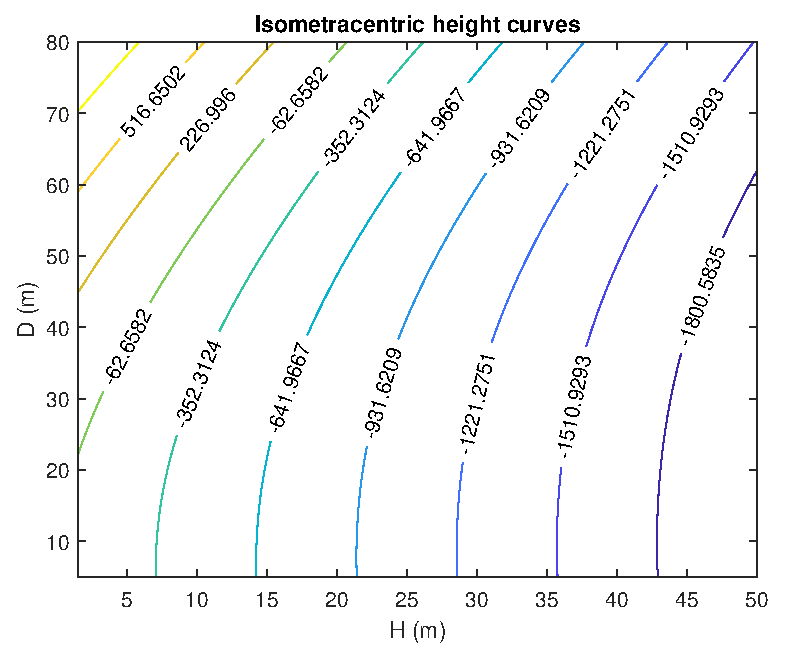
\includegraphics[width=0.8\textwidth]{images/figure_1.eps}
	\caption{La primera figura}
	\label{fig: isom}
\end{figure}
\end{lstlisting}
Generando el siguiente resultado:
\begin{figure}[H]
	\centering
	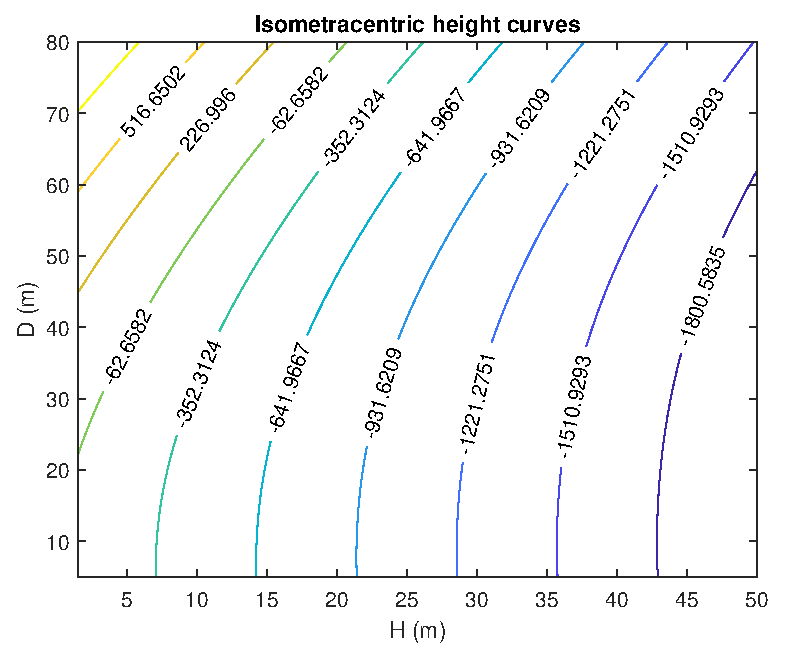
\includegraphics[width=0.8\textwidth]{images/figure_1.eps}
	\caption{La primera figura}
	\label{fig: isom}
\end{figure}

Recuerde insertar gráficas de alta calidad y a ser posible que se contraste bien lo que se quiere mostrar. No todos los documentos son impresos en color pese a las muy altas prestaciones gráficas de hoy en día.


Para colocar varias gráficas, se recurre al entorno \texttt{minipage}. 
\begin{lstlisting}
\begin{minipage}{0.5\textwidth}	
	\begin{figure}[H] 
		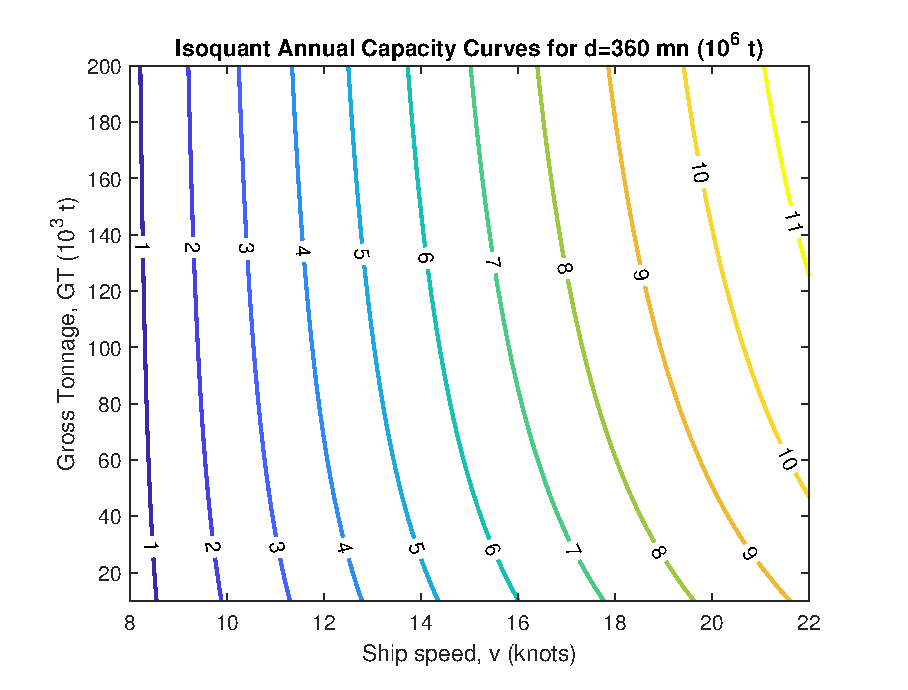
\includegraphics[width=1.00 \textwidth]{images/minipage1.eps}
		\caption{La segunda figura}
		\label{fig: minip}
	\end{figure}	
\end{minipage} \hfill \begin{minipage}{0.5\textwidth}	  
	\begin{figure}[H] 
		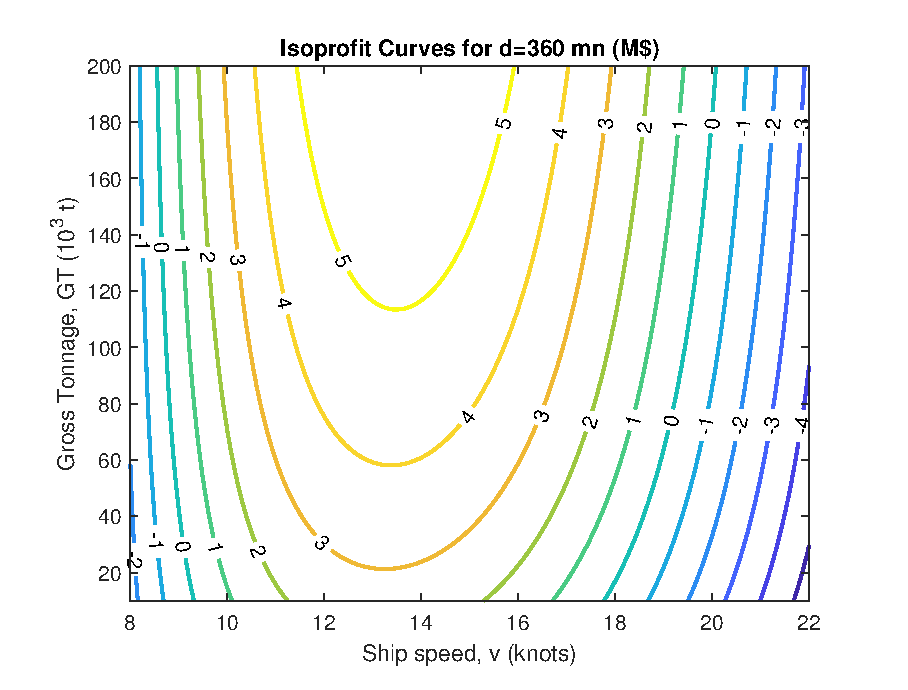
\includegraphics[width=1.00 \textwidth]{images/minipage2.eps}
		\caption{La tercera figura}
		\label{fig: minip2}
	\end{figure}
\end{minipage}
\end{lstlisting}

	\begin{minipage}{0.5\textwidth}	
		\begin{figure}[H] 
		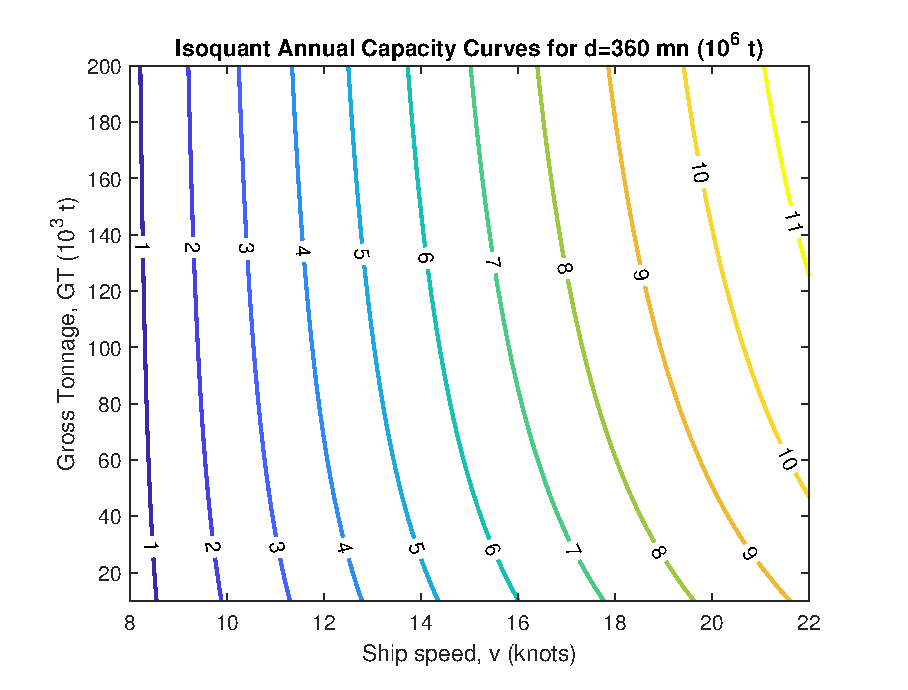
\includegraphics[width=1.00 \textwidth]{images/minipage1.eps}
		\caption{La segunda figura}
		\label{fig: minip}
		\end{figure}	
\end{minipage} \hfill \begin{minipage}{0.5\textwidth}	  
	\begin{figure}[H] 
		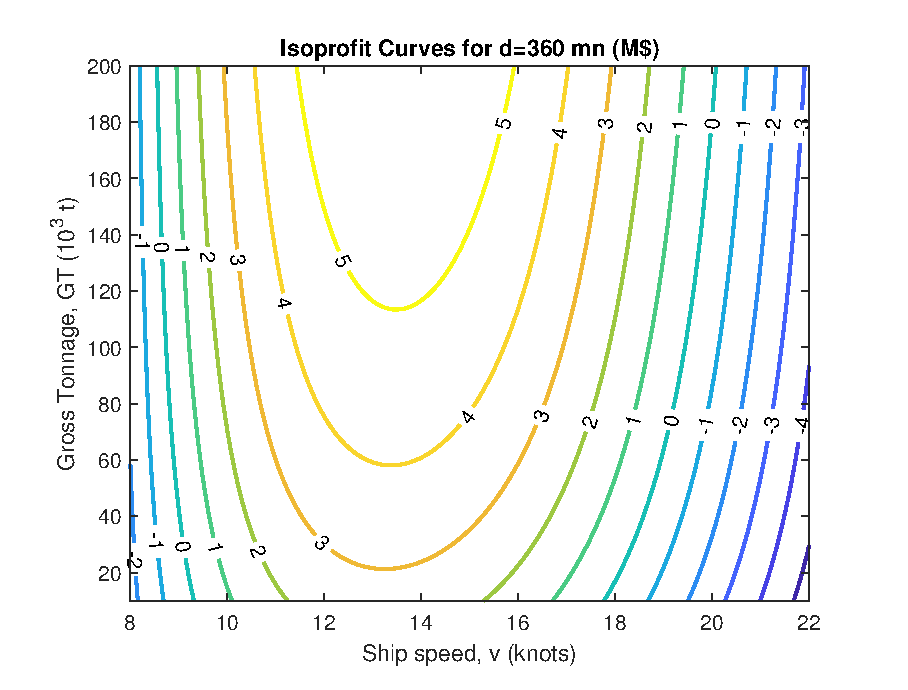
\includegraphics[width=1.00 \textwidth]{images/minipage2.eps}
		\caption{La tercera figura}
		\label{fig: minip2}
	\end{figure}
\end{minipage}


Se recuerda que ambas gráficas deben estar muy relacionadas para mostrarse juntas.
\subsection{Tablas}
Las tablas se numeran también con el número del capítulo seguido del número de tabla en orden creciente. El título está	 centrado y en la parte superior de la tabla. 


Se recomienda que las tablas tengan información concisa y bien estructurada. Sirva el siguiente ejemplo para ilustrar el formato de las figuras:
\begin{lstlisting}
% Table generated by Excel2LaTeX from sheet 'Hoja1'
\begin{table}[H]
\centering
\caption{Principales valores}
\begin{tabular}{lrr}
	\toprule
	Variable   & Valor &   Unidad \\ \midrule
	Potencia   &   1.2 &       MW \\
	Velocidad  &   2.3 &      m/s \\
	Impedancia &   0.3 & $\Omega$ \\ \bottomrule
\end{tabular}%
\label{tab: valores}%
\end{table}%
\end{lstlisting}
% Table generated by Excel2LaTeX from sheet 'Hoja1'
\begin{table}[H]
	\centering
	\caption{Principales valores}
	\begin{tabular}{lrr}
		\toprule
		Variable   & Valor &   Unidad \\ \midrule
		Potencia   &   1.2 &       MW \\
		Velocidad  &   2.3 &      m/s \\
		Impedancia &   0.3 & $\Omega$ \\ \bottomrule
	\end{tabular}%
	\label{tab: valores}%
\end{table}%
Una opción para realizar tablas es utilizar Excel y después generar el código mediante la macro \href{https://ctan.org/pkg/excel2latex?lang=en}{Excel2LaTeX}. Existen opciones similares para LibreOffice.
\subsection{Ecuaciones}
Para las ecuaciones, se pueden escribir en el modo ``en línea''  \lstinline!$c^2=b^2+a^2$!, produciendo el siguiente resultado $c^2=b^2+a^2$ o bien numerándose para luego ser referenciadas (ver Ecuación \ref{eq: ISE}), como se muestra a continuación.

\begin{lstlisting}
	\begin{equation}
	ISE=\int_{0}^{\infty} \left(\widetilde{f}(\tau)-f(\tau)\right) d\tau
	\label{eq: ISE}
	\end{equation}
\end{lstlisting}
\begin{equation}
	ISE=\int_{0}^{\infty} \left(\widetilde{f}(\tau)-f(\tau)\right) d\tau
	\label{eq: ISE}
\end{equation}
Existen numerosos recursos en línea para editar las ecuaciones fácilmente, se recomienda \href{http://www.hostmath.com/}{HostMath}.

\section{Algoritmos}
Para la exposición de un algoritmo u otro procedimiento que se requiera para la puesta en marcha, fabricación, proceso, etc. se puede recurrir al formato que se encuentra en el Anexo \ref{ch: A}. Nótese que no se recomienda incluir código de programación o similares en el cuerpo del documento.
\section{Otros elementos}
Se incluyen aquí otros elementos sujetos a formato como pueden ser los siguientes:


Listas enumeradas
\begin{enumerate}
	\item Primer elemento numerado.
	\item Segundo elemento numerado.
	\item ...
	\item hasta el último
\end{enumerate} 

Viñetas
\begin{itemize}
	\item Primer elemento numerado.
	\item Segundo elemento numerado.
	\item ...
	\item hasta el último
\end{itemize}
    % !TEX encoding = UTF-8 Unicode
% !TEX root = GANXXX.tex
% !TeX spellcheck = es_ES
%%=========================================	
\chapter{Otro capítulo}
Se aprovecha esta sección para dar algunos consejos respecto a la redacción de textos con \LaTeX.
\begin{itemize}
	\item La distribución de \LaTeX usada en este documento es MikTeX 2.9. Se recomienda usar esta versión frente a LiveTeX para evitar posibles errores al compilar.
	\item El compilador es el que trae TeXStudio por defecto: pdfLaTeX.
	\item Un editor muy usado y disponible en Windows, Mac y Linux es TeXstudio. Facilita ciertas operaciones como crear un \texttt{environment}, alineación de tablas, etc. A veces es necesario limpiar los archivos auxiliares que se generan para que el documento se compile más rápido. En TeXstudio, se hace en Tools >  Limpiar archivos auxiliares.
	\item Este documento ha sido dividido en capítulos, por lo que no será necesario compilar todos ellos cuando se esté trabajando en uno. Fácilmente se podrá incluir o no el capítulo usando el comando \lstinline!\include{CapituloX}! en la raíz del documento. Los nombres de los archivos deben NO incluir espacios.
	\item Se deberá hacer referencias a figuras, tablas, ecuaciones o incluso apartados durante el documento. Por ello, es recomendable usar el comando \lstinline!\label{eq: deformada}! para asignar una etiqueta al objeto a referenciar, mientras que usaremos \lstinline!\ref{eq: deformada}! para que se imprima la referencia. Los prefijos ``eq:'', ``fig:'', ``tab'' son muy útiles para no confundir referencias.
	\item Se pueden incluir pies de página\footnote{Tales como éste.} mediante el comando \lstinline!\footnote{Texto que se quiera mostar}! para realizar aclaraciones.
	\item Se recuerda que para poner alguna palabra entre comillas se usarán dos acentos graves al comienzo de la frase (\lstinline!``!) y dos apóstrofos al final (\lstinline!''!).
	\item Para realizar una lista de términos y acrónimos (lo cual se recomienda), una manera alternativa a \lstinline!\makeglossary! es incluir un capítulo sin numeración debajo de ``Agradecimientos'' que se llame ``Términos y Acrónimos'' y pegar una tabla sin bordes que se haya realizado y ordenado alfabéticamente en un Excel. Sería una tabla de dos columnas, con el acrónimo a la izquierda y su definición a la derecha.
\end{itemize}



    % !TeX encoding = UTF-8 Unicode
% !TeX root = GANXXX.tex
% !TeX spellcheck = es_ES
%%=========================================	
\addcontentsline{toc}{chapter}{Información sobre la bibliografía}
\chapter*{Información sobre la bibliografía}
Todos los documentos técnicos (Trabajo Fin de Grado, Tesis Doctoral, Artículo Técnico o Científico, Memoria, etc.) deben incluir una sección de bibliografía en la cual se hace un listado de todas las fuentes consultadas para realizar el trabajo. Es preciso otorgar el crédito a los trabajos realizados por otros y que se utilizan de algún modo u otro en el trabajo propio. Por esta razón, en el texto se deben incluir las referencias a las fuentes empleadas intentando incurrir en plagio, aún cuando ésta no sea nuestra intención. Se citará usando \lstinline!\cite{einstein}! \cite{einstein}.


Todas las fuentes utilizadas deberían ser referenciadas en nuestro trabajo. Estas fuentes pueden ser:

\begin{itemize}
	\item Un libro o capítulo de libro
	\item Un artículo de revista
	\item Un artículo de congreso
	\item Un manual técnico
	\item Un trabajo anterior (Fin de Grado, Fin de Máster, Tesis Doctoral, etc.)
	\item Un enlace virtual (Wikipedia, etc.)
\end{itemize}

Se recomienda usar para la bibliografía programas como ``JabRef'' o ``BibTex'' para gestionar las referencias. El estilo más extendido en publicaciones es el IEEEtran, que en \LaTeX $ $ se denomina \texttt{ieeetr}. Aparecen listados los trabajos a medida que se van citando, tal y como se puede comprobar \cite{knuthwebsite} en la siguiente página. Con este tipo de bibliografía, no aparecerán los trabajos hasta que éstos sean citados.

El siguiente código genera la bibliografía
\begin{lstlisting}
	\bibliographystyle{ieeetr}
	\addcontentsline{toc}{chapter}{\bibname}
	\bibliography{refsreal}  
\end{lstlisting}

	% INCLUIR LOS CAPÍTULOS NECESARIOS
	
	% BIBLIOGRAFÍA
	\bibliographystyle{ieeetr}
	\addcontentsline{toc}{chapter}{\bibname}
	\bibliography{bibliographyfile}

	% ANEXOS
	\begin{appendices}
	\appendixpageoff
	\renewcommand\appendixname{Anexo}
	\renewcommand\chaptername{Anexo}
	\include{AnexA}
    \end{appendices}
\end{document}